% !TEX TS-program = pdflatex
% !TEX encoding = UTF-8 Unicode

% This is a simple template for a LaTeX document using the "article" class.
% See "book", "report", "letter" for other types of document.

\documentclass[11pt]{article} % use larger type; default would be 10pt

%\usepackage[utf8]{inputenc} % set input encoding (not needed with XeLaTeX)

%%% Examples of Article customizations
% These packages are optional, depending whether you want the features they provide.
% See the LaTeX Companion or other references for full information.

%%% PAGE DIMENSIONS

\usepackage{geometry} % to change the page dimensions
\geometry{a4paper} % or letterpaper (US) or a5paper or....
%\geometry{margins=2in} % for example, change the margins to 2 inches all round
% \geometry{landscape} % set up the page for landscape
%   read geometry.pdf for detailed page layout information
\usepackage{fullpage}
%\usepackage[top=tlength, bottom=blength, left=llength, right=rlength]{geometry}
%Edit individual page dimension variables described above, using the \addtolength and \setlength commands. For instance,
%\oddsidemargin=-1cm
%\setlength{\textwidth}{6.5in}
%\addtolength{\voffset}{-5pt}

\usepackage{graphicx} % support the \includegraphics command and options

% \usepackage[parfill]{parskip} % Activate to begin paragraphs with an empty line rather than an indent

%%% PACKAGES
\usepackage{booktabs} % for much better looking tables
\usepackage{array} % for better arrays (eg matrices) in maths
\usepackage{paralist} % very flexible & customisable lists (eg. enumerate/itemize, etc.)
\usepackage{verbatim} % adds environment for commenting out blocks of text & for better verbatim
%\usepackage{subfig} % make it possible to include more than one captioned figure/table in a single float

\usepackage{caption}
\usepackage{subcaption}
\usepackage{cite}
\usepackage{graphicx}
\usepackage{hyperref, amsmath, mathrsfs, bm}

\usepackage{url}
\renewcommand{\thesubfigure}{}
% justifying
\usepackage{ragged2e}


\graphicspath{{./}{./../graphs/}{./graphs/}}


\usepackage{amssymb,amsmath,amsthm,amscd}

\usepackage[mathscr]{eucal}
%\usepackage[dvips]{graphicx}
%\usepackage{pstricks,pst-grad,pst-plot,pst-node}


%\usepackage{pgf}



%\newpsobject{showgrid}{psgrid}{subgriddiv=1,griddots=2,gridlabels=6pt}
\renewcommand{\raggedright}{\leftskip=0pt \rightskip=0pt plus 0cm}
% argmin
\DeclareMathOperator*{\argmin}{arg\,min}

\newcommand{\myred}{\color{red}}
\newcommand{\mygreen}{\color{green!50!black}}
\newcommand{\myblue}{\color{blue}}

\newcommand{\mcX}{\mathcal{X}}
\newcommand{\mcY}{\mathcal{Y}}
\newcommand{\mcG}{\mathcal{G}}
\newcommand{\mcF}{\mathcal{F}}


%\usepackage[tiling]{pst-fill}
\usepackage{epsfig}
\usepackage{graphicx}
\usepackage[usenames,dvipsnames]{color}

\usepackage{Sweave}
\usepackage{tikz}
\usepackage{pgf}

%%% HEADERS & FOOTERS
\usepackage{fancyhdr} % This should be set AFTER setting up the page geometry
\pagestyle{fancy} % options: empty , plain , fancy
\renewcommand{\headrulewidth}{0pt} % customise the layout...
\lhead{}\chead{}\rhead{}
\lfoot{}\cfoot{\thepage}\rfoot{}

%%% SECTION TITLE APPEARANCE
%\usepackage{sectsty}
%\allsectionsfont{\sffamily\mdseries\upshape} % (See the fntguide.pdf for font help)
% (This matches ConTeXt defaults)

%%% ToC (table of contents) APPEARANCE
\usepackage[nottoc,notlof,notlot]{tocbibind} % Put the bibliography in the ToC
\usepackage[titles,subfigure]{tocloft} % Alter the style of the Table of Contents
\renewcommand{\cftsecfont}{\rmfamily\mdseries\upshape}
\renewcommand{\cftsecpagefont}{\rmfamily\mdseries\upshape} % No bold!

\newtheorem{thm}{Theorem}
\newtheorem{cor}{Corollary}
\newtheorem{lem}{Lemma}





%%% END Article customizations

%%% The "real" document content comes below...

\title{ Fidelity-Commensurability tradeoff in Joint Embedding of Disparate Dissimilarities}


%input affiliations


\author{Sancar Adali\thanks{Johns Hopkins University,
Department of Applied Mathematics and Statistics,
100 Whitehead Hall,
3400 North Charles Street,
Baltimore, MD 21218-2682} \and Carey E. Priebe\thanks{Johns Hopkins University,
Department of Applied Mathematics and Statistics,
100 Whitehead Hall,
3400 North Charles Street,
Baltimore, MD 21218-2682}
}
 

% \email{sadali1@jhu.edu}   %optional

% \email{cep@jhu.edu}   %optional
\date {August 1, 2011}% Activate to display a given date or no date (if empty),
         % otherwise the current date is printed 

\begin{document}
\maketitle
\abstract{For matched data from disparate sources (objects observed under different conditions), optimality of information fusion must be defined with respect to the inference task at hand. Defining the task as matched/unmatched hypothesis testing for dissimilarity observations,  Priebe et al.~\cite{JOFC} presents manifold matching using an embedding method based on joint optimization of fidelity (preservation of within-condition dissimilarities between observations of an object) and commensurability (preservation of between-condition dissimilarities between observations) . The tradeoff between fidelity and commensurability is investigated by varying weights in weighted embedding of an omnibus dissimilarity matrix. Optimal (defined with respect to the power of the test) weights for the optimization correspond to an optimal compromise between fidelity and commensurability. Results indicate optimal weights are different than equal weights for commensurability and fidelity and the proposed weighted embedding scheme provides significant improvements in test power.
}




\section{Introduction}

 It is a challenge  to do a tractable analysis on data from disparate sources of data (such as multiple sensors). The multitude  of sensors technology and large numbers of sensors both are  sources of difficulty and hold promise for efficient inference.
 \begin{comment}
 The typical multiple sensor setting is visualized in  Figure ~\ref{fig:fig1}.
\begin{figure}
\centering
\includegraphics[scale=0.75]{gen-model-orig-proj.pdf}
\caption{Multiple Sensor setting}
\label{fig:fig1}
\end{figure}


It is assumed some objects lie in some "object`` space $\Xi$, and each sensor has a distinct "view`` of the objects. The measurements recorded by the $i^{th}$ sensor lie in some "measurement space`` $\Xi_i$. The usual approach in pattern recognition is to extract features from these measurements to get a feature representation in Euclidean space and use classical pattern recognition tools to carry out the exploitation task. The alternative approach is to acquire dissimilarities between the group of objects, and use the dissimilarities to  find an embedding in a low-dimensional Euclidean space where classical statistical tools  can be used.
%, or use these dissimilarities directly if appropriate predictors exist for the dissimilarities and the task .
The embeddings of dissimilarities from  different conditions will be required to be "commensurate`` so that sensor measurements can be compared or jointly used in inference. This is accomplished by maps $\rho_k,k=1,\ldots,K$ from measurement spaces $\Xi_k$ to a low-dimensional commensurate space $\mathcal{X}$ visualized in~\ref{fig:fig1}. Learning these maps from data is  an important portion of the proposed  approach.
\end{comment}
There are quite  a few real life cases, where the data is acquired or available exclusively in dissimilarity representation instead of feature representation~\cite{CMDS,borg+groenen:1997,duin2005dissimilarity}.
 Multidimensional scaling is the processing step used to find the feature representation equivalent of this kind of data, so that  statistial machine learning methods can be applied to the data. A specific variant of MDS will be used to get an embedding in  Euclidean Space. 
 
 In this paper, hypothesis testing is the exploitation task being considered, and   the "optimal'' embedding  refers to  that leads to the  test with  the highest power. Consider the weighted raw-stress function:
\begin{equation}
\sigma_{W}(X)=\sum_{1\leq s\leq n;1\leq t\leq n} {w_{st}(d_{st}(X)-\delta_{st})^2  }\label{raw-stress}
\end{equation}
 for an  $n \times p$ configuration matrix ($n$ points in $p$ dimensions)  $X$  where $d_{st}(X)$ is the Euclidean distance between $s^{th}$ and $t^{th}$ rows of $X$ and $w_{st}$ is the weight for $st^{th}$  squared difference.  $n \times n$  matrix representation of the weights and Euclidean distance will be denoted by $W$ and $D(X)$  , respectively. This   criterion function which will be minimized for embedding configurations is appropriate for the purpose of finding a tradeoff between two different criteria (namely the preservation of fidelity and commensurability).

The dissimilarity-representation version of a hypothesis testing problem is stated as follows:\\
$n$ different objects/instances are measured/judged under $K$ different conditions with (possibly notional) measurements $x_{ik}$ indexed by object and condition. Each of the measurements $x_{ik}$ lies in  the corresponding space $\Xi_k$. 
\[  \begin{array}{cccc}
        & \Xi_1 & \cdots & \Xi_K\\
        Object ~ 1 & \bm{x}_{11} & \sim \cdots \sim & \bm{x}_{1K} \\
        \vdots & \vdots & \vdots & \vdots \\
        %\text{Object} ~ i & \bm{x}_{i1} & \sim \cdots \sim & \bm{x}_{iK} \\
        %\vdots & \vdots & \vdots & \vdots \\
        Object ~ n & \bm{x}_{n1} & \sim \cdots \sim & \bm{x}_{nK}
      \end{array}      
\]
For each pair of measurements $x_{ik},x_{jk}$ in the same space, the dissimilarity value $\delta_{ijk}=\delta\{x_{ik},x_{jk}\}$, is based on the dissimilarity measure on the space $\Xi_k$. The dissimilarities are assumed to be non-negative and  symmetric, and 0 for $\delta\{x_{ik},x_{ik}\}$   . These  dissimilarities are exploited to carry out  the following hypothesis testing task:

 Given dissimilarities between  $K$ new measurements/observations ($\bm{y}_{k};k=1,\ldots,K$) and the previous 
$n$ objects under $K$ conditions,    test the null hypothesis  that ``these measurements are from the same  object"  against the alternative hypothesis that ``they are not  from the same  object"~\cite{JOFC}:
    \[
\begin{array}{l}
%\hspace{-2em}
    H_0: \bm{y}_{1} \sim \bm{y}_{2} \sim \cdots \sim \bm{y}_{K}
 \text{ versus } 
 H_A: \exists i, j , 1\leq i < j \leq K :\bm{y}_{i} \nsim \bm{y}_{j}  
\end{array}
\]
 The null hypothesis can be restated as the case where the dissimilarities are ``matched" and the alternative as the case where they are not ``matched".

Dissimilarities are in the form  of $n \times n$  dissimilarity matrices $\{\Delta_k;k=1,\ldots,K\}$ with entries $\{\delta_{ijk} ;  i=1,\ldots,n;\hspace{5pt} j=1,\ldots,n\}$  and a  vector (of length $nK$) of dissimilarities  $\mathbf{\Delta}^{new}=\{ \delta_{ik}^{new}; i=1,\ldots, n;\hspace{5pt} k=1,\ldots,K\}  $  where $\delta_{ik}^{new} $ is the dissimilarity  between  $x_{ik}$ and $y_k$

 Since dissimilarities are  measured between pairs of objects under the same condition, they will be the entries in  
 separate dissimilarity matrices , each matrix consisting of dissimilarities between pairs of  measurements for a separate condition.
 Due to the fact that data sources are ``disparate", it is not immediately obvious how  a dissimilarity between an object in one condition and another object in another condition  can be computed, or even defined in a sensible way.  In general, these between-condition between-object  similarities are not available. 

Throughout this paper , it will be assumed,  the number of conditions, $K$, is equal to $2$ for the  simplicity of presentation. 

\section{``Matched" and ``Conditions" in data}

 ``Conditions" and ``matched" refer to concepts dependent on the context of the  problem. Conditions could be different modalities of data, e.g., one condition could be  an image of an object, while the other condition could be a text description of the object. ``Matched", in general, means observations of the same object, or realizations of a common concept. 
\section{Two  models for generating data}
In this section, two data models are proposed that illustrate the idea of matchedness.
\subsection{Gaussian setting\label{subsec:GaussianSet}}
	Let    $\Xi_1 = \mathbb{R}^{p}$ and $\Xi_2 = \mathbb{R}^{p}$.
  Let $\bm{\alpha}_i \sim^{iid} MVNormal(\bm{0},I_p)$ represent $n$ ``objects".  Let $\bm{x}_{ik}  \sim^{iid} MVNormal(\bm{\alpha_i},\Sigma)$ represent $K=2$ matched measurements (each under a different condition).
  $\Sigma$ is a positive-definite $p\times p$ matrix such that  $\max(\Lambda(\Sigma))=\frac{1}{r} $ where $\Sigma=U\Lambda(\Sigma)U'$  is the eigenvalue decomposition of $\Sigma$. See Figure~\ref{fig:Fig1}.

The parameter $r$ controls the variability between ``matched" measurements. If $r$ is large, it is expected that the distance between matched measurements
$\bm{x}_{i1}$ and $\bm{x}_{i2}$ to be stochastically smaller than $\bm{x}_{i1}$ and $\bm{x}_{i'2}$ for $i \neq i'$ ; if r is small, then ``matched" is not informative in terms of similarity of measurements.
 Smaller $r$ will make the decision problem harder and will lead to higher rate of errors or tests with smaller power for fixed type I error rate $\alpha$.
  
    \begin{figure}
	\begin{center}
    \includegraphics[scale=0.75]{MVN_alpha_r_multiple_sancar.pdf}
    \caption{For the  Gaussian setting (Section \ref{subsec:GaussianSet}), the $\bm{\alpha_i},$ are denoted by black points and the $\bm{x}_{ik}$ are denoted by red and blue points respectively.}
\label{fig:Fig1}
	\end{center}
  \end{figure}

\subsection{Dirichlet setting\label{subsec:DirichletSet}}
Let $S^p=\{\bm{x}:\bm{x}\in\mathbb{R}^{(p+1)}, \sum_{l=1}^{p+1}{x_l}=1\}$ be the standard $p$-simplex in $\mathbb{R}^{p+1}$.
 Let $\Xi_1 = S^p$ and $\Xi_2 = S^p$.   Denote a vector of ones by $\bm{1}_{p+1}\in \mathbb{R}^{(p+1)}$.
  Let $\bm{\alpha}_i \sim^{iid} Dirichlet(\bm{1}_{p+1})$ represent $n$  ``objects'' and let $\bm{x}_{ik} \sim^{iid} Dirichlet(r\bm{\alpha}_i+\bm{1}_{p+1})$ represent $K$ measurements. 
  %See Figure~\ref{fig:Fig2}.

 The parameter $r$ again controls the variability between ``matched" measurements.
 \begin{comment}
    \begin{figure}
	\begin{center}
    \includegraphics[scale=0.75]{Dirichlet_alpha_r_multiple_sancar.pdf}
   \caption{ For the  Dirichlet setting (Section \ref{subsec:DirichletSet}),  the $\bm{\alpha_i},$ are denoted by black points and the $\bm{x}_{ik}$ are denoted by red and blue points respectively.}
\label{fig:Fig2}
	\end{center}
  \end{figure}
\end{comment}
\subsection{Noise\label{noise}}
Measurements $\bm{x}_{ik}$ carry the signal that is relevant to the exploitation task.  Noise dimensions can be introduced to  the measurements by concatenating a $q$-dimensional error vector whose magnitude is controlled by the parameter $c, c\in (0,1)$. The noisy measurements will be  represented by the random vectors 
 \begin{equation}
\breve{X}_{ik}=[(1-c)\bm{x}_{ik}\hspace{5pt} cE_{ik}]\label{eq:noise-expr}
\end{equation}
 where $E_{ik} \sim^{iid} Dirichlet(\bm{1}_{(q+1)})\label{eq:noise-model-dir} $ for the Dirichlet setting and $E_{ik} \sim^{iid} MVNormal(\bm{0} , (1+\frac{1}{r})I_{q+1}) \label{eq:noise-model-mvn} $ for the Gaussian setting. $\breve{X}_{ik}$ will be used instead of $\bm{x}_{ik}$ for computing dissimilarities in the ``noisy" version of the problem. These noisy measurements allow the comparison of  different methods applied to the problem with respect to their robustness.
  

\section{Manifold Matching\label{sec:JOFC}}
  The JOFC approach can be summarized as identifying embeddings of multiple disparate data sources into the same low-dimensional space where joint inference can be pursued. 

It  will be assumed  the commensurate space  $\mathcal{X}$  is  $\mathbb{R}^d$ where $d$ is pre-specified. The selection of $d$ -- model selection -- is  a task that requires much attention and is  beyond the scope of this article. Discussion of the effect of $d$ on matching performance will be available at a later paper.

To embed dissimilarities  $\{\Delta_k,k=1 ,\ldots,K\}$  from different conditions into a commensurate space in one step, an omnibus dissimilarity matrix  $M$ can be embedded in the low-dimensional Euclidean spaceinto one omnibus dissimilarity matrix $M$, imputing entries if necessary. Consider, for $K=2$, \begin{equation}
M=  \left[ \begin{array}{cc}
         \Delta_1 & L\\
        L^T  & \Delta_2 
     \end{array}  \right]     \label{omnibus} 
\end{equation} where $L$ is a matrix of imputed entries. One way to impute $L$ is to set it to $\frac{\Delta_1+\Delta_2}{2}$. Another choice for imputation is introduced in \ref{sec:FidComm}: the diagonal of $L$ is set to 0, the rest of the entries are $NA$ and are ignored in the optimization of MDS criterion.  
Using MDS to embed  this omnibus matrix into a  space  $\mathcal{X}$,  $2n$ embedded observations $\{\tilde{y}_i^{(k)}; i=1,\ldots,n;k=1,2\}$ are obtained in a single space, with distances between the different observations consistent with the given dissimilarities. Now that the observations are commensurate, it is possible to  compute the test statistic \[
\tau=d\left(\tilde{y}_i^{(1)},\tilde{y}_j^{(2)}\right)\label{teststat}
\] for $i^{th}$ and $j^{th}$ observations under different conditions.  For ``large" values of $\tau$, the null hypothesis will be rejected. This approach will be referred to as the Joint Optimization of Fidelity and Commensurability (JOFC) approach, for reasons that will be explained in Section \ref{sec:FidComm}. 
  Out-of-sample extension for MDS will be used throughout this paper\cite{TrossetOOS}. 

% - given the embedded configuration $X$ of the 
%training observations and the augmented dissimilarity matrix that includes dissimilarities between test observations and %the training observations, and dissimilarities in between the training observations, oos-embedding consists of embedding
%the test points into  the existing configuration so as to be as consistent as possible with these dissimilarities (the distances %between points are as close as possible to the dissimilarities as measured by the criterion function). 


\section{Fidelity and Commensurability constraints for Manifold Matching \label{sec:FidComm}}
Unless 
\begin{itemize}
\item the dissimilarity matrix is the Euclidean distance matrix of the original observations, and, 
\item the embedding dimension is greater or equal to the dimension of the original observations,
\end{itemize}
MDS with raw stress will not result in a perfect reconstruction  of the original observations. Note that the objective of the embedding is not \emph{perfect} reconstruction, but the best embedding for the exploitation task which is to test whether two sets of dissimilarities are ``matched". What is considered a good ``commensurate" representation will be dependent on how well the information in original dissimilarities that is relevant to the the match detection task is preserved. The following two criteria  embody the two kind of information  that is relevant to this task.


\begin{itemize}
\item Fidelity is how well the mapping to commensurate space preserves the original dissimilarities. The loss of \em{fidelity} can be measured with  within-condition \em{ fidelity error} is given by
    \[
\epsilon_{f_{k}} = \frac{1}{{{n}\choose{2}}} \sum_{1 \leq i < j \leq n} (d(\widetilde{\bm{x}}_{ik},\widetilde{\bm{x}}_{jk})-\delta_k(\bm{x}_{ik},\bm{x}_{jk}))^2
\] 
where ${\bm{x}}_{ik}$ is the original observation of the $i^{th}$ object for the $k^{th}$  condition and $\widetilde{\bm{x}}_{ik}$ is the embedded configuration of the $i^{th}$ object  for the $k^{th}$ condition;  $d(\cdot,\cdot)$ is the Euclidean distance function (for the embedding space) and $\delta_k(\cdot,\cdot)$ is the dissimilarity function defined for objects in the $k^{th}$ condition.

\item Commensurability is how well the mapping to commensurate space preserves matchedness of matched observations. The loss of commensurability can be measured by the between-condition {\em commensurability error} is given by
    \[
\epsilon_{c_{k_1k_2}} = \frac{1}{n} \sum_{1 \leq i \leq n;k_1 <k_2} (d(\widetilde{\bm{x}}_{ik_1},\widetilde{\bm{x}}_{ik_2})-{ \delta_{k_1k_2}}(\bm{x}_{ik_1},\bm{x}_{ik_2}))^2
\label{comm-error}
\]
 for conditions $k_1$ and $k_2$; $\delta_{{k_1}{k_2}}(\cdot,\cdot)$ is the (notional) dissimilarity function between measurements in  $k_1^{th}$ and $k_2^{th}$ conditions. Note that ,in general, there are $K$  within-condition fidelity error terms and $\frac{K \times (K-1)}{2}$  between-condition commensurability error terms.


Although  the between-condition dissimilarities of the same object, ${ \delta_{k_1k_2}(\bm{x}_{ik_1},\bm{x}_{ik_2}})$, are not available,  it is not unreasonable in this setting  to set ${ \delta_{k_1k_2}}(\bm{x}_{ik_1},\bm{x}_{ik_2}) = 0$ for all $i,k_1,k_2$.  So diagonal  entries of $L$ in  equation \eqref{omnibus} are  chosen to be all zeroes. Setting these diagonal entries to zero forces matched points to be embedded close to each other.

Then, the commensurability error  term becomes
  \[
\epsilon_{c_{k_1k_2}} = \frac{1}{n} \sum_{1 \leq i \leq n;k_1< k_2} (d(\widetilde{\bm{x}}_{ik_1},\widetilde{\bm{x}}_{ik_2})))^2
\]
\end{itemize}

 There is also between-condition {\em separability error} given by
    $$\epsilon_{s_{k_1k_2}} = \frac{1}{{{n}\choose{2}}} \sum_{1 \leq i < j \leq n;k_1 <k_2} (d(\widetilde{\bm{x}}_{ik_1},\widetilde{\bm{x}}_{jk_2})-{ \delta_{k_1k_2}}(\bm{x}_{ik_1},\bm{x}_{jk_2}))^2.$$ This error will be ignored herein, due to the fact that 
$\delta_{k_1k_2}(\bm{x}_{ik_1},\bm{x}_{jk_2})$ is not  available. 

In the  raw stress version of  MDS,  the individual terms can be separated according to whether they are contributing to  fidelity or  commensurability  error.

 Consider the weighted raw stress criterion $\sigma_{W}(\cdot)$ with a weighting matrix $W$, given in equation~\eqref{raw-stress}.

\begin{align}
\sigma_W(\cdot)  &= & &\sum_{i,j,k_1,k_2} {w_{ij{k_1}{k_2}}(d_{ij{k_1}{k_2}}(\cdot)-M_{ijk_1k_2})^2 } \notag\\
\hspace{3pt} &=& &\underbrace{\sum_{i=j,k_1<k_2}  {w_{ij{k_1}{k_2}}(d_{ij{k_1}{k_2}}(\cdot)-M_{ijk_1k_2})^2}}_{Commensurability}  \hspace{10pt}  &  + &\hspace{2.5em} \underbrace{\sum_{i<j,k_1=k_2}  {w_{ij{k_1}{k_2}}(d_{ij{k_1}{k_2}}(\cdot)-M_{ijk_1k_2})^2  }  } _{Fidelity}\notag\\
\hspace{3pt}&+&  &\underbrace{\sum_{i< j,k_1<k_2}  {w_{ij{k_1}{k_2}}(d_{ij{k_1}{k_2}}(\cdot)-M_{ijk_1k_2})^2  }  } _{Separability}\label{eq:FidCommSep}\hspace{10pt} .
\end{align}


Since ${ \delta_{k_1k_2}}(\bm{x}_{ik_1},\bm{x}_{ik_2}) $ are set to 0, the corresponding entries of $M$ in the commensurability terms will be 0.

Since    the separability error is ignored,  the weights for separability terms are chosen to be 0. This also means off-diagonal elements of $L$ in equation \eqref{omnibus} can be ignored. When separability terms are removed from equation \eqref{eq:FidCommSep}, the resulting equation  is a sum of fidelity and commensurability error terms:


\begin{align}
\sigma_W(\cdot)\hspace{3pt}   
\hspace{3pt}&=&\underbrace{\sum_{i=j,k_1< k_2}  {w_{ij{k_1}{k_2}}(d_{ij{k_1}{k_2}}(\cdot))^2}}_{Commensurability}  \hspace{10pt}  &  +&\underbrace{\sum_{i< j,k_1=k_2}  {w_{ij{k_1}{k_2}}(d_{ij{k_1}{k_2}}(\cdot)-M_{ijk_1k_2})^2  }  } _{Fidelity}\notag\label{eq:FidCommSep}\hspace{10pt} .
\end{align}

This motivates  referring to the omnibus embedding approach as Joint Optimization of Fidelity and Commensurabilty (JOFC).

\subsection{Alternative Methodologies}

Two alternative methodologies exist that correspond roughly to the extreme ends of the range of $w$ values
For the optimization of commensurability with fidelity as  secondary priority($w\approx 1$), an alternative method is Canonical Correlational Analysis (CCA)~\cite{Hardoon2004}, which aims to find linear subspaces of the Euclidean space  such that the projection of data points to those subspaces results in  vectors that are maximally correlated. For the optimization of fidelity ,  one can use Principal Components Analysis (PCA), which aims to find linear subspaces such that  projection of data points to those subspaces results in observation vectors that represent the original data as best as possible. To optimize commensurability as  secondary priority, one can use the projections computed by PCA to  compute a Procrustes transformation that will make the projections commensurate. This $Procrustes \circ MDS$ approach is   analagous to $w\approx 0$ case for JOFC. Details about these methodologies along with the exact nature of relationship to extreme ends of JOFC will be discussed in another paper.


\section{Related Work \label{sec:RelatedWork}}
There have many efforts toward solving the related problem of ``manifold alignment".``Manifold alignment" seeks to find correspondences between observations from different ``conditions". The setting that is most similar to ours is the semi-supervised setting\cite{Ham}, where a set of correspondences are given and the task is to find correspondences between a new set of points in each condition. In contrast, the hypothesis testing task discussed in this paper is to determine whether any given pair of points is ``matched" or not. The proposed solutions follow a common approach in that they look for a common commensurate or a latent space, such that the representations (possibly projections or embeddings) of the observations in the commensurate space match.\cite{Wang2008,Zhai2010,3wayNMDS}


\section{Fidelity and Commensurability Tradeoff}
The major question  addressed in this work is whether in the tradeoff between preservation of fidelity and preservation of  commensurability , there is an optimal point for the match detection task.  The weights in raw stress allow us to answer this question relatively easily. Since in equation \eqref{eq:FidCommSep},  each term indexed with $i$, $j$ is either a fidelity or a commensurability term, setting $w_{ij}$ to $w$ and $1-w$  for commensurability  and fidelity  terms respectively will allow us to control the importance of fidelity and commensurability terms in the optimization by varying $w$. 
\begin{align*}
\sigma_W(X)&=  f_w(D(X),M) & &\\
&=  \underbrace{\sum_{i=j,k_1\neq k_2}  {w(d_{ij{k_1}{k_2}}(X))^2}}_{Commensurability} & +\hspace{2em} & \underbrace{\sum_{i<j,k_1=k_2}  {(1-w)(d_{ij{k_1}{k_2}}(X)-M_{ijk_1k_2})^2  }  } _{Fidelity}\\
&=  \left(w\right)\left(n\right) \epsilon_{c_{k_1=1,k_2=2}} & +\hspace{2em} & (1-w){{n}\choose{2}} ( \epsilon_{f_{k=1}}+\epsilon_{f_{k=2}} )
\end{align*}

The expectation here is that there is a $w^*$ that is optimal for the specific exploitation task (has the best power in hypothesis testing). In fact,  exploratory simulations presented in this paper confirm the power of the tests varies with varying $w$ and indicate the range where the optimal  $w^*$ lies.



\section{Definition of  $w^{*}$}
Two dissimilarity matrices are defined to be $\Delta^{(m)} \left(\left[
\begin{array}{c}
\mathcal{T} \\
X_{1}^{(m)} \\
X_{2}^{(m)} 
\end {array}
\right]
\right)$  and 
 $\Delta^{(u)} \left(\left[
\begin{array}{c}
\mathcal{T}\\
X_{1}^{(u)} \\
X_{2}^{(u)}
\end {array}
\right]\right)$ as two matrix-valued random variables $\Delta^{(m)}:\Omega \rightarrow \mathbf{M}_{n\times n} $,$\Delta^{(u)}:\Omega \rightarrow \mathbf{M}_{n\times n} $  for the appropriate sample  space $(\Omega)$. These dissimilarity matrices are result of dissimilarities between    an i.i.d sample of  matched measurements  augmented with  a matched and unmatched pair of measurements respectively. 

 The criterion function for the embedding is $\sigma_W(\cdot) =f_w(D({\cdot}),\Delta)$. All of the random variables following the embedding is dependent on $w$, for the sake of simplicity, it will not be shown in the notation. The embedding for the unmatched pair ${\hat{X}_{1}^{(u)},\hat{X}_{2}^{(u)}}$  is 
 \[
{\hat{X}_{1}^{(u)},\hat{X}_{2}^{(u)}}
=\argmin_{\acute{X}_{1}^{(u)}, \acute{X}_{2}^{(u)}}\left[\min_{\mathbf{\acute{T}}}
{f_w\left(
D\left(
\left[
\begin{array}{c}
\acute{\mathbf{T}} \\
\acute{X}_{1}^{(u)} \\
\acute{X}_{2}^{(u)}
\end {array}
\right]
\right),
\Delta^{(u)}
\right)
}
\right]
\]
where there is an implicit dependence on $\mathbf{T}$, because $\Delta^{(u)}$ depends on $\mathbf{T}$. 
A similar expression gives the embedding for the matched pair  
${\hat{X}_{1}^{(m)},\hspace{0.5em}\hat{X}_{2}^{(m)}}=\argmin_{\acute{X}_{1}^{(m)}, \acute{X}_{2}^{(m)}}\left[\min_{\mathbf{\acute{T}}}
{f_w\left(
D\left(
\left[
\begin{array}{c}
\acute{\mathbf{T}} \\
\acute{X}_{1}^{(m)} \\
\acute{X}_{2}^{(m)}
\end {array}
\right]
\right),
\Delta^{(u)}
\right)
}
\right]$.
 Assuming these minima exist and are unique, the mappings $\hat{X}_{1}^{(m)}:\omega\rightarrow \mathbf{R}^{d'}$,  $\hat{X}_{2}^{(m)}:\omega\rightarrow \mathbf{R}^{d'}$ , $\hat{X}_{1}^{(u)}:\omega\rightarrow \mathbf{R}^{d'}$, 
$\hat{X}_{2}^{(u)}:\omega\rightarrow \mathbf{R}^{d'}$ are  measurable maps,  $\hat{X}_{1}^{(m)}$ , $\hat{X}_{2}^{(m)}$ , $\hat{X}_{1}^{(u)}$, $\hat{X}_{2}^{(u)}$ are random vectors. 

Consider the test statistic $\tau=d(\hat{X}_{1}^{\cdot},\hat{X}_{2}^{\cdot})$. Under null hypothesis of matchedness, the distribution of the statistic is governed by the distribution of $\hat{X}_{1}^{(m)}$ and $\hat{X}_{2}^{(m)}$, under the alternative it is governed by  $\hat{X}_{1}^{(u)}$ and $\hat{X}_{2}^{(u)}$.

Denote by $F_Y$ the   cumulative distribution function of  $Y$ where $Y$ can be  any function of $\hat{X}_{k}^{(m)}$ or $\hat{X}_{k}^{(u)}$.  for $k=\{1,2\}$ 



 Then $$\beta_{\alpha}\left( w\right)=1-F_{d \left(\hat{X}_{1}^{(u)},\hat{X}_{2}^{(u)}\right)}(F_{d\left(\hat{X}_{1}^{(m)},\hat{X}_{2}^{(m)}\right)}^{-1}(1-\alpha)).$$

 Note that all random variables are dependent on $w$. Finally, define $$w^{*}=\arg\max_w{\beta_{\alpha}\left( w\right)}. $$


Even for  given $\mathbf{F}_u,\mathbf{F}_m$,   $w^*$ must be defined with respect to the value of allowable type I error rate $\alpha$.  For two different $\alpha$ values, it is quite possible that $\beta_{\alpha_1}(w_1)>\beta_{\alpha_1}(w_2)$  and $\beta_{\alpha_2}(w_1)<\beta_{\alpha_2}(w_2)$. This can be observed in results in Section \ref{sec:Simulation Results}.  
Investigation of some  properties of $w^{*}$  is included in section  \ref{sec:Simulation Results} .
 $w^*$ is defined to be the argmin of  the power function with respect to $w$ and some important questions about $w^*$ are  related to the nature of this function $\beta_{\alpha}\left( w\right)$.
While finding an analytical expression for the value of $w^*$ is intractable, an estimate $\hat{w}^*$  based on noisy evaluations of $\beta_{\alpha}(w^*)$ can be computed.  A Monte Carlo simulation is run in  Section  \ref{sec:Simulation Results} 
to find the estimate of $\beta_{\alpha}\left( w\right)$ at various values of $w$ and $\alpha$ .

\begin{comment}
A closed-form expression for this function will be hard to find  even in the most simple of cases. So consider the estimate from the Monte Carlo simulation $\beta^{(m)}_{\alpha}(w)$ for the estimate computed from $2m$ testing pairs, m matched pairs and m unmatched pairs. In addition, consider an arbitrary element $\omega$ of sample space $\Omega$. By law of large numbers, $\beta^{(m)}_{\alpha}\rightarrow\beta_{\alpha}(w)$ pointwise.  We will omit $w$ from the expressions of the functions. Suppose the test statistic values  are $T_0^{i}$, $T_A^{i}$ $i=1,\ldots,m$  respectively for matched and unmatched test pairs. Note that $\beta^{(m)}_{\alpha}$ can be written as $\sum_{j=1}^m I(T_A^{j}>T_0^{(i)})$ where $T_0^{(i)}$ is the $i=\lceil {m*(1-\alpha)} \rceil^{th}$ order statistic of $T_0^{i},i=1,\ldots,m$. Replacing the indicator function with the unit step function
\[
\beta^{(m)}_{\alpha}=\sum_{j=1}^m u(T_A^{j}-T_0^{(i)})
\]

Instead of this function which is not differentiable with respect to  $T_0^{i}$ and  $T_A^{i}$, consider the ``soft" approximation of this function with the sigmoid function
\[
\mathcal{B}_{alpha}^{(m)}=\sum_{j=1}^m \sigma(T_A^{j}-T_0^{(i)})
\]

Now we can consider the derivative  $\frac{d\mathcal{B}_{\alpha}^{(m)}}{dw}$, which is equal to 
\[
\frac{d\mathcal{B}_{\alpha}^{(m)}}{dw}=\sum_{j=1}^m \frac{\partial \sigma(T_A^{j}-T_0^{(i)})}{\partial T_A^{j}} \frac{\partial T_A^{j}}{w}+ \sum_{j=1}^m \frac{\partial \sigma(T_A^{j}-T_0^{(i)})}{\partial T_0^{j}} \frac{\partial T_0^{j}}{\partial w}
\] if the partial derivatives exist.
To prove differentiability of $\beta_{\alpha}\left( w\right)$ , we refer to Theorem 5.3.3 in \cite{ElClassAnalysis-5-3-3}, which requires the pointwise convergence of   $\mathcal{B}_{alpha}^{(m)}$   to  $\beta_{\alpha}\left( w\right)$ , that $\frac{d\mathcal{B}_{alpha}^{(m)}}{dw}$ are continuous and that they  converge \emph{uniformly} to a function $g$. Since the sigmoid function $\sigma(\cdot)$ is continously differentiable, we can focus on our attention  on $ \frac{\partial{T_0^{j}}}{\partial{w}}$ and $ \frac{\partial{T_0^{j}}}{\partial{w}}$. We show  that while the embedded configurations of points might not be  continuous everywhere (we present a particular example in \ref{subsubsec:Discontinuity}) $T_0^{j}$ and $T_A^{i}$ is nevertheless continuous with respect to $w$. 
\end{comment}


 
\subsection{Continuity of $\beta(\cdot)$} 
 Let $T_0(w)$ and $T_a(w)$ denote the value of the test statistic under null and alternative distributions  for the embedding with $w$ .  %stochastic process whose sample path is  a function of $w$ where the randomness comes from $\Delta^{(m)}$, $\Delta^{(u)}$ and %$\mathcal{T}$ . 
Consider $\beta_{\alpha}(\cdot)$ as a function of $w$, which can be written as $P\left[T_a(\cdot)>c_{\alpha}(\cdot)\right]$ where $c_{\alpha}(\cdot)$ is the critical value for level $\alpha$. Instead of  $\beta_{\alpha}(\cdot)$

  the area under the curve measure will be shown to be continuous as a surrogate: $$AUC(w)=P\left[T_a(w)>T_0(w)\right]$$ where $T_a(\cdot)$ and $T_0(\cdot)$ can also be regarded as  stochastic processes whose sample paths are continuous functions of $w$ except at a finite number of points in $(0,1)$.


\begin{thm}
Let $T(\cdot)$ be  a stochastic process indexed by $w$ in the interval (0,1). Assume  the process is continuous in probability  (stochastic continuity)   everywhere in the interval  i.e.
$$ \forall a>0 \quad  \lim_{\delta \rightarrow 0} Pr\left[\|T(w+\delta)-T(w) \|>a \right] \rightarrow 0 \quad(*)$$ 

 $\forall w\in (0,1)$.

Then,

for any $w>0, \epsilon>0$, there exist $\delta_{\epsilon}$ $$\| Pr\left[T(w+\delta_{\epsilon})>0 \right]- Pr\left[T(w)>0 \right]\|<\epsilon .  $$

and 

$Pr \left[ T(w)>0\right]$ is continuous with respect to $w$.
\end{thm}

\begin{proof}
 . For any  $\delta$ for which $\delta+w \in (0,1)$, consider the difference of the probabilities of the two events  $T(w)>0$ and $T(w+\delta)>0$ for any $w$.
 \hspace{-1in}
 %\begin{center}
\begin{eqnarray*}
\| Pr\left[T(w+\delta)>0\right]- Pr\left[T(w)>0 \right]\| & = & \| Pr\left[T(w+\delta)>0   \cap T(w) \leq 0 \right] + Pr\left[T(w+\delta)>0   \cap T(w) > 0 \right] - \\
& & (Pr\left[T(w+\delta)> 0   \cap T(w) > 0 \right]+ Pr\left[T(w+\delta)\leq 0  \cap T(w) > 0\right]\| \\
& = & \| Pr\left[T(w+\delta)>0   \cap T(w) \leq 0 \right]- Pr\left[T(w+\delta)\leq 0  \cap   \leq 0 \right]Pr\left[T(w) \leq 0 \right]-\\
& &  Pr\left[T(w+\delta)\leq 0  | T(w) > 0\right]Pr\left[T(w) > 0 \right]\| \\
& \leq &  \max ( Pr\left[T(w+\delta)>0   | T(w) \leq 0 \right]Pr\left[T(w) \leq 0 \right] ,\\
& & Pr\left[T(w+\delta)\leq 0  | T(w) > 0\right]Pr\left[T(w) > 0 \right] ) \\
& \leq &  \max ( Pr\left[T(w+\delta)>0   | T(w) \leq 0 \right] ,\\
& & Pr\left[T(w+\delta)\leq 0  | T(w) > 0\right]) \\
& \leq &  \max ( Pr\left[T(w+\delta)>0   | T(w) \leq 0 \right] ,\\
& & Pr\left[T(w+\delta)\leq 0  | T(w) > 0\right]) 
\end{eqnarray*} 
%\end{center}
For any $w$, choose $\delta_{\epsilon}$ such that such that both $ Pr\left[T(w+\delta_{\epsilon})>0   | T(w) \leq-+ 0 \right] <\epsilon$ and  $Pr\left[T(w+\delta_{\epsilon})\leq 0  | T(w) > 0\right]<\epsilon $. Such a value of  $\delta_{\epsilon}$  exists , since the conditional probabilities $Pr\left[T(w+\delta)>0   | T(w) \leq 0 \right]$ and $ Pr\left[T(w+\delta)\leq 0  | T(w) > 0\right]$  can be made smaller than $\epsilon$ due to stochastic continuity. Therefore 
\[2
\| Pr\left[T(w+\delta)>0\right]- Pr\left[T(w)>0 \right]\| \leq \max ( Pr\left[T(w+\delta)>0   | T(w) \leq 0 \right] , Pr\left[T(w+\delta)\leq 0  | T(w) > 0\right]) <\epsilon 
\]
Therefore $ Pr\left[T(w)>0\right]$ is continuous with respect to $w$.

\end{proof}
Theorem 2.1 in \cite{Norkin1993} states the same theorem :  if $T(w,\omega)$ is continuous with respect to $w$  almost everywhere 
($Pr[\omega:T(w,\omega)\textrm{ is discontinuous with respect to } w]=0$  where $\omega \in \Omega$, and $\Omega$ is the sample space)
, then $F(x)=Pr\left[T(w)>0\right]$ is continuous.

\begin{cor}{
 $AUC(w)=P\left[T_a(w)-T_0(w) >0 \right]$ is continuous with respect to $w$.}
\end{cor}
\begin{proof}
 $Pr\left[T(w)>0 \right]$  as a function of $w$ is continuous with respect to $w$.  Let $T(w)=T_a(w)-T_0(w)$.
\end{proof}



\begin{comment}
First, note that  $\beta(w)$ is continuous with respect to $w$ and locally convex  with respect to embedding coordinates $\hat{X}_{.}$
\end{comment}

\section{Simulation Results\label{sec:Simulation Results}}
To compare the  different approaches, training data of matched sets of measurements were generated according to the Dirichlet and Gaussian settings. Dissimilarity representations were computed from pairwise Euclidean distances of these measurements. A set of matched pairs and unmatched pairs of measurements were also generated for testing with the same distributions. Following the out-of-sample embedding of the dissimilarities test pairs (computed via by one of the three P$\circ $M, CCA and JOFC approaches)  test statistics  for matched and unmatched pairs were used to compute power values at a set of fixed type I error rate $\alpha$ values.

 Additionally, to take robustness of methods into consideration, ``noisy" measurements were created from the original measurements by concatenating randomly generated independent noise vectors (subsection \ref{noise}).  The magnitude of noise is controlled by the parameter $c$ in equation \eqref{eq:noise-expr}). The original setting, with $c=0$,  will be referred as the ``noiseless case".
If the magnitude of noise is small enough, and the embedding dimension is not larger than signal dimension, the embeddings provided by PCA and MDS will not be affected significantly. However  if the number of noisy dimensions (controlled by the parameter $q$ in the distribution of $E_{ik}$ as defined in equation \eqref{eq:noise-expr}) is large enough, embeddings via  CCA  will be affected due to spurious correlation between noisy dimensions.

Given the setting ("Gaussian","Dirichlet"),   the steps for each Monte Carlo replicate are as follows:
\begin{itemize}
\item A training set ($\mathbf{T}_{mc}$) which consists of  $n$ pairs of matched measurements is generated.  If $c=0$, the ``noiseless" data setting is being simulated and measurements are $p$-dimensional vectors, otherwise  the ``noisy" setting is being used to generate data and measurement vectors are $(p+q)$-dimensional. $ \mathbf{T}_{mc}$ = 
$\begin{array}{ccc}
        X_{11} & \ldots & X_{1K} \\
        \cdots & \cdots      & \cdots   \\ 
        X_{n1} & \ldots     & X_{nK} \\
    \end{array}
$
 where each $X_{ik}$ is a random vector of dimension $(p+q \times I(c>0))$ and the conditional distribution  $X_{i.}|\bm{\alpha}_i  $ is specified as an appropriate Multivariate Normal or Dirichlet distribution.
\item Dissimilarities are computed and embedded in  Euclidean space  via MDS (followed by a transformation from  $\mathbf{R}^d$ to  $\mathbf{R}^d$ and  projection into $\mathbf{R}^d$, respectively  for P$\circ$M and CCA) . The final embeddings lie in $\mathbb{R}^d$.   Denote this in-sample embedding configuration as   $\hat{\mathbf{T}}$. Note that  if the JOFC method is being used, embedding is carried out with the weighted raw stress function $\sigma_{W}(\cdot)=f_{w}(D(\cdot),M)$ in equation \eqref{fid-comm-tradeoff-func} with a common weight $w$ for commensurability terms and another common weight $1-w$ for fidelity terms, otherwise unweighted raw stress function ($\sigma(\cdot)$) is used as a criterion function for embedding.

\item  $m$ pairs of matched   measurements are generated which are treated as out-of-sample, and 
\begin{itemize}
\item compute the dissimilarities  %$\mathbf{\Delta}^{new}={ \delta_{ik}^{new}; i=1,\ldots, n;\hspace{5pt} k=1,2}$
 between these out-of-sample  points and the points in ${\mathbf{T}_{mc}}$,  
\item  embed the OOS dissimilarities as pairs of embedded points via the OOS extension:\\
 $(\tilde{y}_1^{(1)},\tilde{y}_1^{(2)}),\ldots, (\tilde{y}_m^{(1)},\tilde{y}_m^{(2)})$, 
\item compute the test statistic $\tau$ for each pair.%, $t(\tilde{y}_i^{(1)},\tilde{y}_i^{(2)});\hspace{4pt}
%i=1,\ldots,m$
\end{itemize}
 The values of the statistic $\tau$ are used for computing  the empirical cumulative distribution function under null hypothesis. 

\item Identical steps for $m$ pairs of unmatched measurements result in the empirical cumulative distribution  function of $\tau$ under alternative hypothesis.
\item For any fixed $\alpha$ value, a critical value for the test statistic and the corresponding power is computed.
\end{itemize}

\begin{figure}
 \centering
  \captionsetup[subfigure]{subrefformat=parens,labelformat=parens}
        \begin{subfigure}[b]{0.45\textwidth}        
              \includegraphics[scale=0.35]{MVN-FC-Tradeoff-OOS-c0_01.pdf}
                \caption{Power ($\beta$) vs Type I error ($\alpha$) plot for different $w$ values for the Gaussian setting (noisy case)}
               
                \label{fig:MVN-c001-power-alpha}
        \end{subfigure}%
        \begin{subfigure}[b]{0.5\textwidth}        
           \includegraphics[scale=0.35]{MVN-FC-Tradeoff-OOS-c0.pdf}
\caption{Power ($\beta$) vs Type I error ($\alpha$) plot for different $w$ values for the Gaussian setting (noiseless case)}
\label{fig:MVN-c0-power-alpha}
        \end{subfigure}%
        
         \begin{subfigure}[b]{0.45\textwidth}  
         \includegraphics[scale=0.95]{OOSMVN-power-w-c0_01.pdf}
\caption{Power ($\beta$) vs $w$ plot for different Type I error ($\alpha$) values for the Gaussian setting (noisy case)}
\label{fig:MVN-c001-power-w}
         \end{subfigure}%
         \begin{subfigure}[b]{0.5\textwidth} 
\includegraphics[scale=0.95]{OOSDirichlet-power-w-c0-01.pdf}
\caption{Power ($\beta$) vs $w$ plot for different Type I error ($\alpha$) values for the Dirichlet setting (noisy case)}
\label{fig:Dir-c001-power-w}
  \end{subfigure}%
  
          \begin{subfigure}[b]{0.5\textwidth}  
\includegraphics[scale=0.35]{Dirichlet-FC-Tradeoff-OOSc0-01-n150.pdf}
\caption{Power ($\beta$) vs Type I error ($\alpha$) plot for different $w$ values for the Dirichlet setting (noisy case)}
\label{fig:Dir-c001-power-alpha}
  \end{subfigure}%  
  \begin{subfigure}[b]{0.45\textwidth} 
  \includegraphics[scale=0.35]{Dirichlet-FC-Tradeoff-OOSc0-n150.pdf}
\caption{Power ($\beta$) vs Type I error ($\alpha$) plot for different $w$ values for the Dirichlet setting (noiseless case)}
\label{fig:Dir-c0-power-alpha}
  \end{subfigure}
  
  \caption {ROC curves and $\beta$ vs $w$ plots for simulation experiments}
  \end{figure}




Setting p and q to 5 and 10, respectively, for $n=150$ and $m=150$, the average of the power values for $nmc=150$ Monte Carlo replicates are computed at  different $\alpha$s and are plotted in Figure \ref{fig:MVN-c001-power-w} against $\alpha$ for the Gaussian setting.  Qualititatively similar plots for the Dirichlet setting  are not included for brevity.  The plot in Figure \ref{fig:MVN-c001-power-w} shows that for different values of  $w$, $\beta$-$\alpha$ curves vary significantly.  The conclusion is that the match detection tests with JOFC embedding using specific $w$ values have better performance than other $w$ values in terms of power.  In Figure
 \ref{fig:MVN-c001-power-w},  $\beta(w)$ is plotted against $w$ for fixed values of $\alpha$. It is  interesting that the optimal value of $w$ seems to be in the range of $(0.85,1)$ for all settings, which suggests a significant emphasis on commensurability might be  critical for the match detection  task. 




\begin{comment}
\begin{figure}
\includegraphics[scale=0.35]{OOS-MVN-power-w-c0.pdf}
\caption{$\beta$ vs $w$ plot for fixed $\alpha$ values for the Gaussian setting (noiseless case)}
\label{fig:MVN-c0-beta-w}
\end{figure}


\begin{figure}
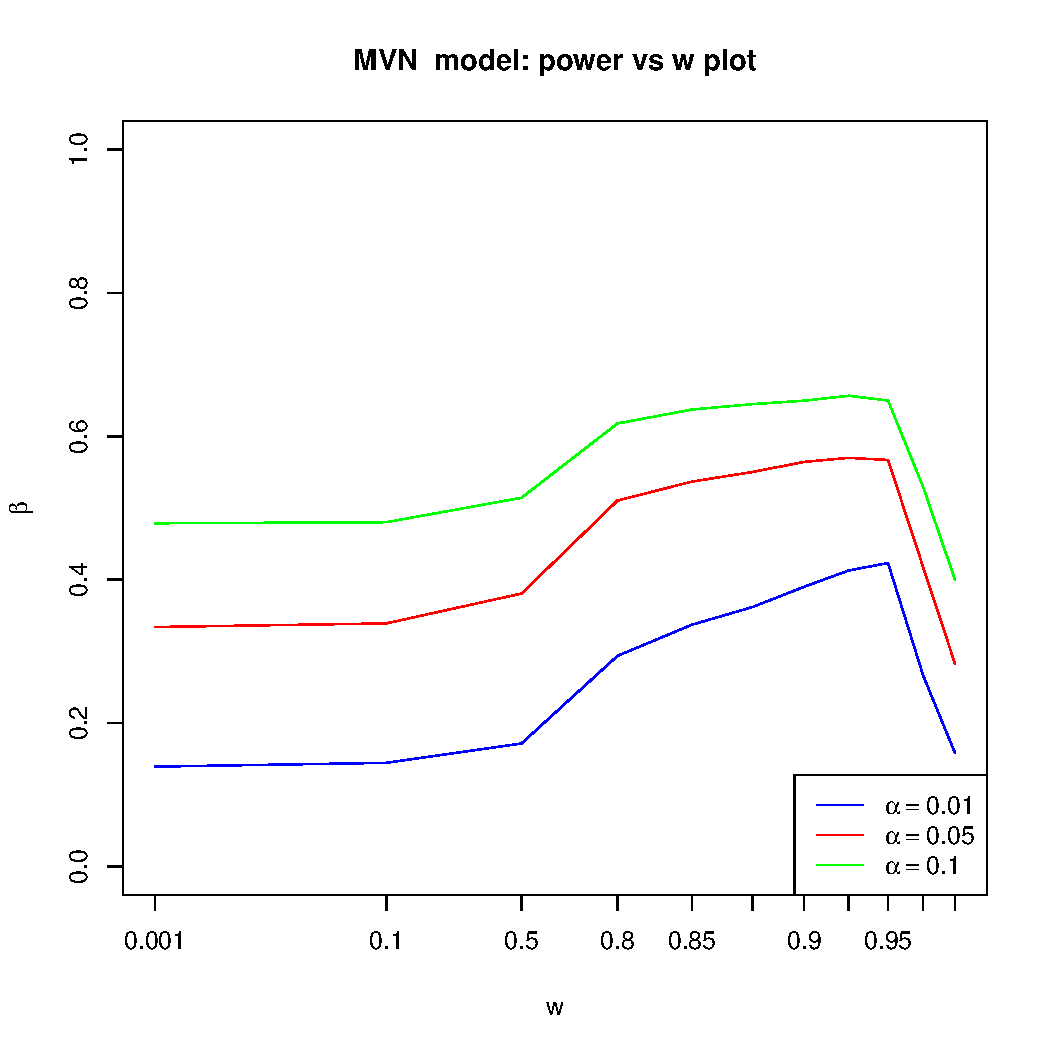
\includegraphics[scale=0.65]{OOSMVN-power-w-c001.pdf}
\caption{Power ($\beta$) vs $w$ plot for fixed Type I error ($\alpha$) values for the Gaussian setting (noisy case)}
\label{fig:MVN-c001-beta-w}
\end{figure}

\end{comment}

Note that in Figure \ref{fig:MVN-c001-power-w} for $\alpha=0.05$, $\beta_{\alpha=0.05}(w=0.99)\geq\beta_{\alpha=0.05}(w=0.5)$. However, for $\alpha=0.3$, $\beta_{\alpha=0.3}(w=0.99)\leq\beta_{\alpha=0.3}(w=0.5)$. This justifies our comment that  $w^{*}$  must be defined with respect to $\alpha$.


\begin{comment}
\begin{figure}
\includegraphics[scale=0.35]{OOS-Dirichlet-power-w-c0.pdf}
\caption{$\beta$ vs $w$ plot for fixed $\alpha$ values for the Dirichlet setting(noiseless case)}
\label{fig:fig7}
\end{figure}

\begin{figure}
\includegraphics[scale=0.35]{OOS-Dirichlet-power-w-c0-01.pdf}
\caption{$\beta$ vs $w$ plot for fixed $\alpha$ values for the Dirichlet setting(noisy case)}
\label{fig:fig8}
\end{figure}
\end{comment}



Note that  for all of the settings, the estimate of the optimal $w^{*}$ has  higher power than $w$=0.5 (the unweighted case).
To test the statistical significance of this observation,   the null hypothesis that  $H_{0}: \beta_{\alpha}({\hat{w}^*})\leq\beta_{\alpha}({w=0.5})$  is tested against the alternative $H_{A}=\beta_{\alpha}({\hat{w}^*})>\beta_{\alpha}({w=0.5})$.  The least favorable null hypothesis is that  $H_{0}: \beta_{\alpha}({\hat{w}^*})=\beta_{\alpha}({w=0.5})$.
Using previous notation,  the test statistic will be denoted by $T_a(w)$ under the alternative hypothesis and $T_0(w)$ under the null hypothesis.

McNemar's test will be used to compare the two predictors (referred to as $C_1$ and $C_2$ with $w$=0.5 and $w$=$w^*$ at a fixed $\alpha$ value.

For the noisy version of the Gaussian setting at allowable type I error 0.05 for the two tests, when comparing  the null hypothesis that  $H_{0}: \beta_{\alpha}({\hat{w}^*})=\beta_{\alpha}({w=0.5})$ against the alternative $H_{A}=\beta_{\alpha}({\hat{w}^*})>\beta_{\alpha}({w=0.5})$, the p-value is $p<1.09E-24$ which indicates the power using estimate of optimal $w^*$ is significantly greater than the power when using $w=0.5$. 
%In fact
% the distribution of p-values from McNemar's tests is skewed and  we reject $\beta_{0.5}>=\beta_{w^*} $ for  55\%  of the %Monte Carlo replicates.

\begin{comment}



\section{Model Selection}
For the simulations presented up to now, the embedding dimension $d$ was set to 2. This was a convenient choice which allowed us to investigate various aspects of JOFC and competing approaches.
However,  more care is required in selection of this parameter, since it plays such a big role in performance in general learning settings. The signal dimension was set to $p=10$ and different $d=2,5,7,10,15$ values were used to test the JOFC approach.
The following plots of ROC curves in    \ref{fig:ROC-d} and  \ref{fig:ROC-d-15} shows the effect of $d$ parameter on the performance of different methods for the Gaussian setting for the noisy case. 
\begin{figure}
 \centering
  \captionsetup[subfigure]{labelformat=empty}
        \begin{subfigure}[b]{0.5\textwidth}        
               \includegraphics[width=\textwidth]{ROC-d-2.pdf}
                \caption{d=2}
                \label{fig:ROC-d-2}
        \end{subfigure}%
         %add desired spacing between images, e. g. ~, \quad, \qquad etc. 
          %(or a blank line to force the subfigure onto a new line)
        \begin{subfigure}[b]{0.5\textwidth}           
                  \includegraphics[width=\textwidth]{ROC-d-5.pdf}
                \caption{d=5}
                \label{fig:ROC-d-5}
        \end{subfigure}      
        %add desired spacing between images, e. g. ~, \quad, \qquad etc.    %(or a blank line to force the subfigure onto a new line)
        \begin{subfigure}[b]{0.47\textwidth}             
               \includegraphics[width=\textwidth]{ROC-d-7.pdf}
                \caption{d=7}
                \label{fig:ROC-d-7}
        \end{subfigure}          
               \begin{subfigure}[b]{0.47\textwidth}
                \centering
               \includegraphics[width=\textwidth]{ROC-d-10.pdf}
                \caption{d=10}
                \label{fig:ROC-d-10}
        \end{subfigure}
        
          \begin{subfigure}[b]{0.47\textwidth}
             \centering
               \includegraphics[scale=0.3]{ROC-d-15.pdf}
                \caption{d=15}
                \label{fig:ROC-d-15}
                        \end{subfigure}
         
        \caption{Effect of $d$ parameter on ROC plots}\label{fig:ROC-d}
        \label{fig:ROC-d}

\end{figure}


\end{comment}

\section{Conclusion}
 The tradeoff between Fidelity and Commensurability and the relation to the weighted raw stress criterion for MDS were both investigated with several simulations and experiments on real data.
   For  hypothesis testing as the exploitation task, the three approaches were compared in terms of testing power.
    The results indicate that the joint optimization (JOFC) approach is superior to CCA and  P$\circ$M,
     and is also robust to spurious correlations CCA suffers from.
      Also when doing a joint optimization, one should consider an optimal compromise point between Fidelity and Commensurability,
       which corresponds to an optimal weight $w^*$ of the weighted raw stress criterion in contrast to the unweighted raw stress 
        for omnibus matrix embedding. 
        The JOFC approach is quite versatile and can be applied to many problems where data of multiple modalities have to be made commensurate. 
        JOFC approach was also applied to  test for matches between Wiki articles and pairs of vertices in random graph data.  Performance of JOFC in these simulations and experiments shows that it 
        it is an appropriate method for these settings.  



\bibliographystyle{plain}
\bibliography{priebe-thesis-JOFC}



\end{document}
